% sec_lambda.tex
\section{Длина свободного пробега и структура СЭ}

Попробуем оценить величину значения длины свободного пробега частиц СЭ \(\lambda_{\text{сэ}}\) между парами последовательных соударений. Разобьём интервал возможных значений длины свободного пробега \(\lambda_{\text{сэ}}\) от \(0\) до \(d_a\) на \(M \to \infty\) равных частей и представим произвольное \(\lambda_n\) в виде
\[
\lambda_n = \frac{n}{M} d_a,
\]
где \(n\) принимает значения от \(1\) до \(M\). Выберем произвольный объём СЭ, содержащий \(N \to \infty\) частиц. Сопоставим каждой частице длину свободного пробега согласно представленной процедуре. Очевидно, что в силу изотропности и стационарности процесса столкновений частиц количество совпадающих по величине значений длин свободного пробега будет одинаковым для каждого \(\lambda_n\) из выбранного нами разбиения. Пусть это будет \(K\) совпадений, при этом \(N = K \times M\). Для вычисления применим классическое определение среднего значения применительно к длине свободного пробега частицы СЭ:
\[
\langle\lambda_{\text{сэ}}\rangle = \frac{\sum_{n=1}^{M} K \lambda_n}{N} = \frac{\sum_{n=1}^{M} K \cdot \frac{n}{M}d_a}{KM} = \frac{d_a}{M^2} \sum_{n=1}^{M} n = \frac{d_a}{M^2} \cdot \frac{M(M+1)}{2} \approx \frac{d_a}{2}.
\]

Полученное значение интуитивно было вполне ожидаемо и вместе с тем «псевдожидкость» свободного эфира представляет собой весьма плотно упакованную среду с очень насыщенным кинетическим потенциалом, по типу нагретого до очень большой температуры газа в замкнутом сосуде, образно и по сути — «всемогущий джин в бутылке».

%\begin{figure}[h]
%\centering
%\includegraphics[width=0.3\textwidth]{images/Столкновение.png}
%\caption{Диаграмма скольжения в различных системах координат.}
%\label{fig:sliding_diagrams}
%\end{figure}

%Для полноты восприятия процесса соударения Амеров СЭ и ЭВ в режиме \textbf{скольжения} на рис. \ref{fig:sliding_diagrams} приведены диаграммы их скоростей в различных системах координат: (а) — абсолютная система координат; (б) — система, связанная с движением центра масс \(\mathbf{v}_{\text{цм}}\); (в) — соударение относительно Амера СЭ; (г) — соударение относительно Амера ЭВ.

\begin{figure}[h]
\centering
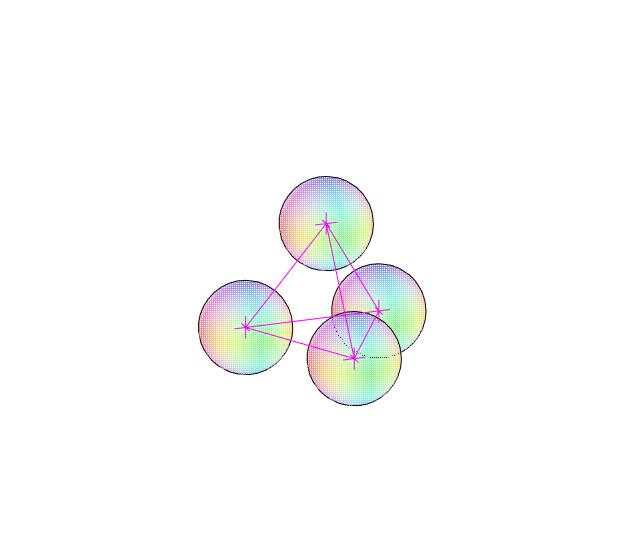
\includegraphics[width=0.25\textwidth]{images/a19.png}
\caption{Пространственное расположение Амеров в СЭ.}
\label{fig:amers_arrangement}
\end{figure}

Рис. \ref{fig:amers_arrangement} даёт наглядное представление о взаимном пространственном расположении Амеров в СЭ в свете полученной оценочной величины длины их свободного пробега в сравнении с диаметром частицы \(d_a\). Автор намеренно изображает наименьшее количество Амеров, показывая этим ограниченные возможности частиц к совершению перемещений, одновременно обозначая способ упаковки пространства движущимся эфиром в дальнейших исследованиях, а именно используя форму тетраэдра, предложенную Платоном в глубокой древности именно для характеристики эфира.

Nieco dalej, ale kontynuując: Небольшое значение длины свободного пробега частиц \(\langle\lambda_{\text{сэ}}\rangle \approx d_a/2\) w СЭ указывает na to, że ich пространственная миграция вследствие хаотических столкновений не может быть значительной, а в пределах нескольких актов соударений будет одного порядка с \(d_a\), в том числе в окрестности граничной поверхности ЭВ. Таким образом, в силу ограничений, связанных со структурной организацией СЭ, составляющие его частицы ведут довольно «оседлый» образ жизни, что позволяет использовать эту особенность для оценки параметров эфирной среды, составляющей тело ЭВ. Рассмотрим отдельный акт соударения двух частиц эфира в режиме \textbf{скольжения}. Амер СЭ после столкновения с наибольшей вероятностью начнёт движение вдоль оси соударения в направлении вектора граничной поверхности \(\mathbf{n}\) (рис. \ref{fig:sliding_diagrams}(а)) со скоростью \(\|\mathbf{v}_{\text{сэ}}\|\) и совершит перемещение величиной, равной среднему значению длины свободного пробега в СЭ, т.е. \(d_a/2\). В конце перемещения он, по определению, сталкивается с другим Амером СЭ и начинает двигаться, предположительно, в обратном направлении. Конечно, он не возвратится в точку первого соударения, но можно утверждать, что это будет её окрестность. Предположим идеальный вариант, в результате которого, совершив обратное перемещение длиной \(d_a/2\) со скоростью \(\|\mathbf{v}_{\text{сэ}}\|\), Амер вернулся на исходную позицию на граничной поверхности. Во время его отсутствия в течение \(d_a / \|\mathbf{v}_{\text{сэ}}\|\) это место на границе было не занято, так как движения Амеров СЭ вдоль граничной поверхности ЭВ нет, и столкновений с Амерами ЭВ также не могло быть, а значит, столкновение произойдёт примерно в момент возврата Амера СЭ на исходное место. Обратная последовательность событий для Амера ЭВ, участвующего в столкновении, предполагает обязательное выполнение некоторых условий, без которых соударение не могло произойти. Вектор скорости \(\mathbf{v}_{\text{эв}}\) Амера ЭВ перед столкновением должен иметь соответствующее направление (рис. \ref{fig:sliding_diagrams}(а)), что предполагает предшествующее соударение с аналогичным Амером ЭВ в потоке, в результате которого произошёл соответствующий «обмен» хаотическими компонентами \(\mathbf{v}\) в соответствии с уравнением \(\mathbf{v}_{\text{эv}} = \mathbf{v}_n + \mathbf{v}\). Однако, чтобы получить соответствующий импульс в процессе столкновения, Амер ЭВ перед этим также должен обладать скоростью определённой направленности, вероятнее всего, полученной в результате предыдущего столкновения на границе ЭВ \(\mathbf{v}_{\text{эв}}'\) (рис. \ref{fig:sliding_diagrams}(а)). В пользу такого сценария развития событий служит «скользящий» характер движения Амеров ЭВ параллельно граничной поверхности. Однако надо признать, что эти предположения не являются бесспорными и являются, в какой-то степени, данью уважения к авторитету Николы Теслы и его предположению о «газоподобности» ЭВ. Тем не менее искомый сценарий, реализующий на границе ЭВ равенство потоков импульса и отсутствие взаимопроникновения Амеров СЭ и ЭВ, возможен пока в двух вариантах. В излагаемом варианте, когда \(n_{\text{сэ}} > n_{\text{эв}}\), где поток частиц в ЭВ обладает свойствами газа, а значит, сжимаем, и \(\|\mathbf{v}_n\| \gg \|\mathbf{v}\|,\|\mathbf{v}_{\text{сэ}}\|\), что открывает широкие вариативные возможности поведения газокинетических материальных систем в части осуществления причинных источников процессов, лежащих в основе известных и неизвестных видов взаимодействий между материальными вихревыми объектами и системами. Однако выполнение указанных требований к эфирокинетической системе ЭВ вызывает ряд вопросов, связанных с физической возможностью их осуществления в процессе образования вихря, который предполагает пространственную сепарацию частиц эфира по видам движения, а также скоростям направленных потоков, в результате чего возникает газообразное фазовое состояние эфира. Надо отметить, что СЭ, являясь весьма плотной средой, не обладает наличием каких-либо связей между частицами, а значит, отсутствует возможность существования состояний эфира, из которых он в каких-либо особых условиях может переходить в газообразное состояние, когда длина свободного пробега частиц значительно превышает их диаметр. Подобный переход возможен как результат процесса распада эфирокинетической системы, находящейся в неравновесном состоянии, представленной, например, практически одномоментно завихренной «псевдожидкостью» СЭ. Процесс организованной трансформации первоначального вихревого образования, безусловно, очень интересная тема, достойная в дальнейшем отдельного исследования; однако неравномерное распределение количества движения по сечению потока, связанное с особенностью пространственного строения тора, неизбежно приводит либо к одномоментной, либо к цепной трансформации (что не суть важно) последовательности коаксиально расположенных поверхностных разрывов и фрагментации первоначального направленного потока эфирной «псевдожидкости» на слои, разделённые направленными потоками газообразного эфира — \textbf{каналами (Кn)}. Коаксиальная фрагментация первоначального вихря естественным образом сопровождается перетоками импульса через все граничные поверхности, которых у каждого вихревого потока эфирного газа-канала ровно две. В результате этих перетоков некоторые слои «псевдожидкого» эфира внутри ЭВ, вероятнее всего, возвратятся в первоначальное хаотическое состояние, утратив направленность в движении, а во внутренней осевой части вихря сформируется «кольцевая зона» эфирной «псевджидкости», которую В.А. Ацюковский называл \textbf{керном}, а автор взял на себя смелость назвать \textbf{«Несвободным эфиром» (НЭ)}.

\begin{figure}[h]
\centering
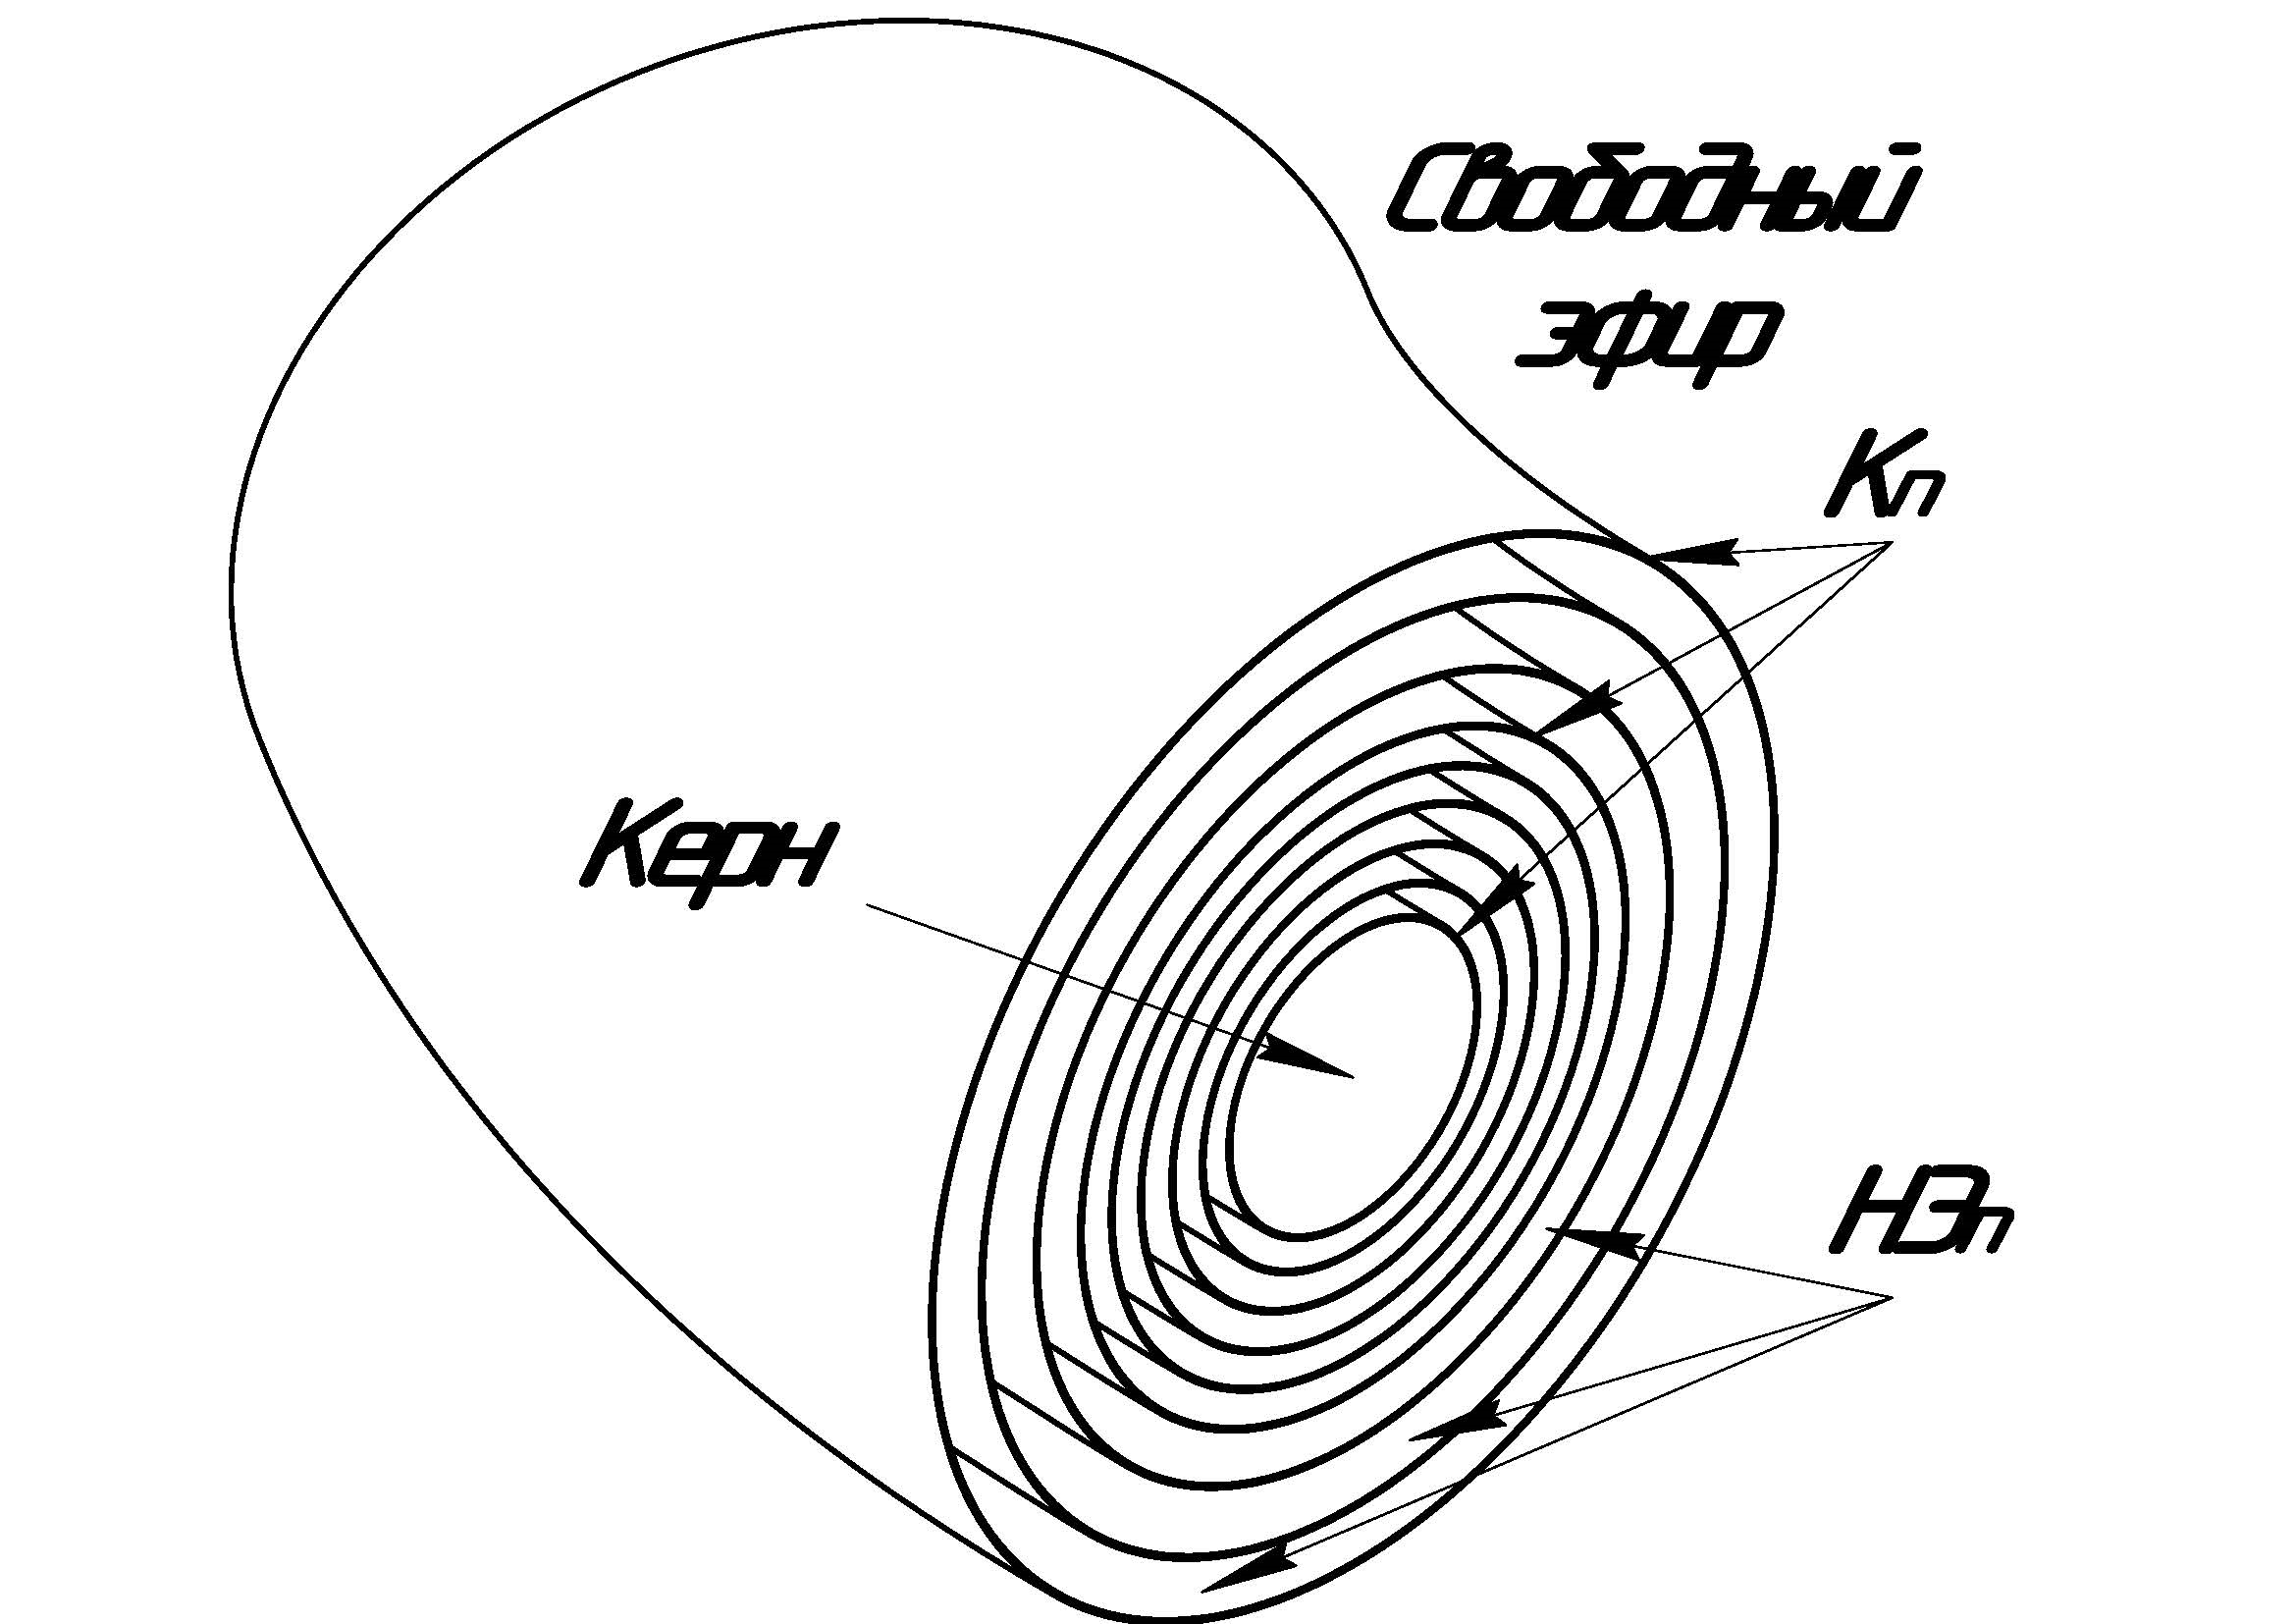
\includegraphics[width=0.4\textwidth]{images/a6.png}
\caption{Схема коаксиальной структуры ЭВ.}
\label{fig:coaxial}
\end{figure}

Осуществление такого сценария формирования эфирного вихря с точки зрения физики процесса выглядит достаточно искусственным, так как возникновение газового направленного потока частиц эфира между двумя граничными поверхностями означает необходимость значительного превышения скорости направленного движения Амеров в канале над скоростью частиц эфира в соседних областях НЭ. Это условие возникает из необходимости поддержания баланса импульса и числа столкновений на каждой из двух граничных поверхностей при том, что концентрация частиц в газовой фазе эфира много меньше концентрации частиц в СЭ и НЭ. Абсолютная упругость и парность столкновений частиц эфира исключают физическую возможность возникновения у какой-либо из них скорости, значительно отличающейся от величины среднего значения. То же самое справедливо для процесса возможного изменения скорости частиц эфира в сторону меньших значений. Косвенным подтверждением такого предположения о внутренней структуре ЭВ служит приведённая ниже теневая фотография газового вихря (рис. \ref{fig:gas_vortex}), к которой автор в дальнейшем будет апеллировать, аргументируя существование физических аналогий у фундаментальных свойств вещественной материи.

\begin{figure}[h]
\centering
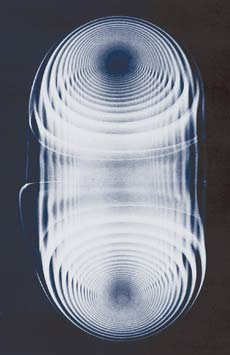
\includegraphics[width=0.2\textwidth]{images/a12.png}
\caption{Теневая фотография газового вихря (аналогия).}
\label{fig:gas_vortex}
\end{figure}

Более вероятный сценарий осуществления «долгоживущих» вихревых эфирных структур возможен при \(n_{\text{сэ}} = n_{\text{эв}}\), что также позволяет реализовать равновесный процесс перетока импульса через граничную поверхность ЭВ, если среднее значение длины свободного пробега Амера в направленном потоке эфира вихря \(\lambda_{\text{эв}} \approx d_a/2\), которое можно трактовать как \textbf{«правило запрета на обгон»}, при этом \(\|\mathbf{v}_n\| > 2\|\mathbf{v}\|\), что означает неизменность направления потока частиц. Равенство концентраций частиц в обоих фазовых состояниях эфира на граничной поверхности может указывать на то, что «слоистая» структура эфирного вихревого объекта формируется во время процесса его образования, а не как результат последующей за ним цепочки событий. Коаксиальная вложенность вихревых \textbf{эфирных каналов (Кп)}, разделённых областями \textbf{несвободного эфира (НЭ)}, которыми также заполнено центральное осевое пространство полнотория, является принципиальным атрибутом внутренней структуры каждого вихревого эфирного объекта весомой материи. Вихри могут отличаться геометрическими размерами, количеством \textbf{каналов}, но всегда присутствуют \textbf{внутреннее осевое кольцо (керн)}, вокруг которого совершается непрерывный процесс вихревого направленного движения, а также наружная «упаковка» из \textbf{Свободного} или \textbf{Несвободного эфира}, обеспечивающая кинетику вихревого движения и пространственную целостность объекта весомой материи. Таким образом, эфирные вихревые объекты весомой материи или, другими словами, \textbf{элементарные частицы} и \textbf{фотоны} представляют собой пространственные «наборы» из дискретных вихревых элементов в виде \textbf{каналов}, которые в классической физике можно соотносить с \textbf{квантами}. Таким образом совершенно естественно возникло квантовое обустройство элементарных частиц и фотонов и физическая основа \textbf{квантовой механики}. Пространственно ориентированные вихревые эфирные каналы — прекрасные объекты для вычисления спинов или моментов объектов весомой материи. Коаксиальная структура вихревого эфирного объекта весомой материи допускает \textbf{одновременное сосуществование разнонаправленных вихревых каналов} в одном объекте. Маловероятно, что разнонаправленность вихревых потоков может возникать в процессе «рождения» элементарной частицы; однако такой сценарий может быть реализован при взаимодействии элементарных частиц, поглощении и испускании фотонов. \textbf{Дискретная структура вихревых эфирных объектов весомой материи является необходимым условием для их осуществления}, что является отражением взаимной обусловленности параметров СЭ и ЭВ и детерминированностью процессов на границе раздела фазовых состояний эфира.

\begin{figure}[h]
\centering
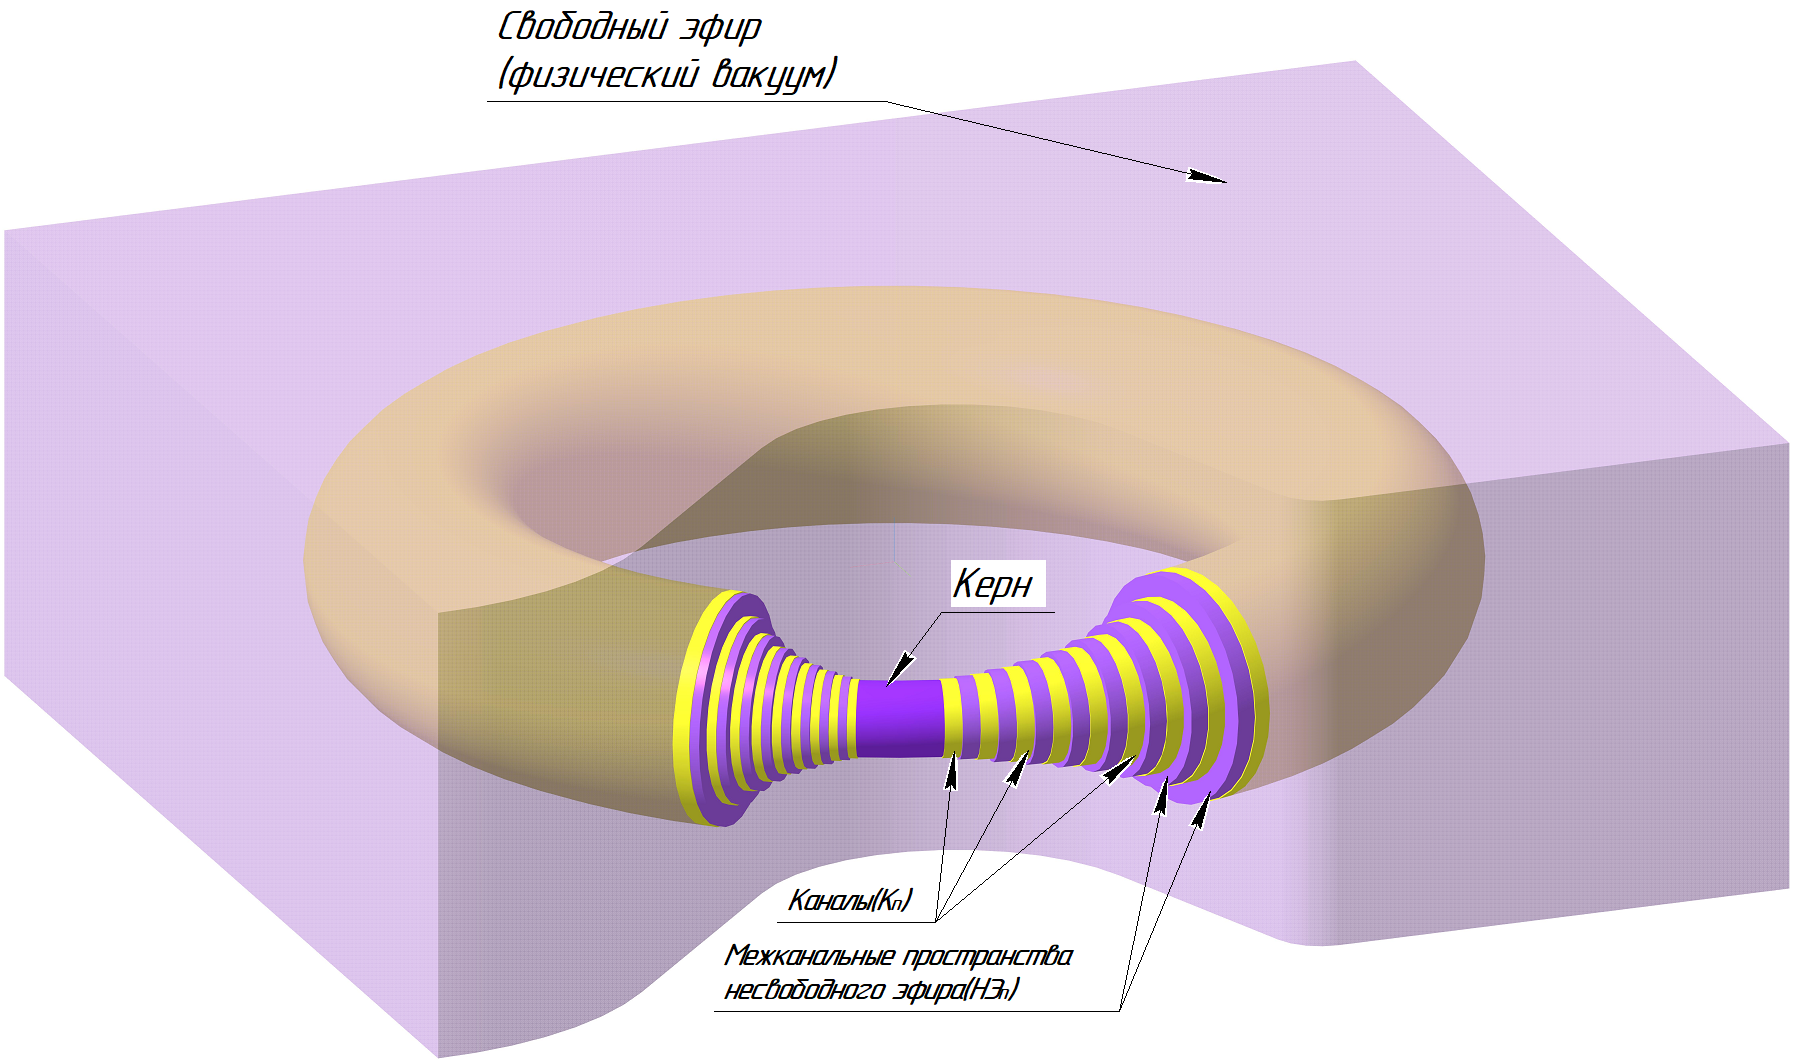
\includegraphics[width=0.55\textwidth]{images/a29.png}
\caption{Упрощённая схема структуры вихревого эфирного объекта весомой материи.}
\label{fig:vortex_structure}
\end{figure}

На рис. \ref{fig:vortex_structure} приведена упрощённая схема структуры вихревого эфирного объекта весомой материи. Объект намеренно изображён погружённым в среду Свободного эфира с целью подчеркнуть его особую роль в процессе его физического осуществления. В дальнейшем, в целях упрощения, Свободный эфир изображаться не будет, за исключением случаев, когда в этом будет необходимость.
